
\paragraph{Monkeys exhibit hallmarks of color category behavior}

The animals examined show a hallmark of color categorization behavior: memory biases towards a set of particular points in a perceptually uniform colorspace.
In \autoref{fig:BiasCurves} it can be seen that the biases deviate substantially and systematically from zero, with the attractor points being found where the bias line crosses the zero line from positive to negative (going counter-clockwise). These points are highlighted with colored lines, with the filled areas around these lines showing the confidence intervals on these crossing points. Repeller points found where the line crosses the zero line from negative to positive.

\begin{figure}
%\includesvg[inkscapelatex=false, height=\textwidth]{../../Figures/F3_BiasCurves_v2.svg} % this is messing up currently for unknown reasons
\begin{center}
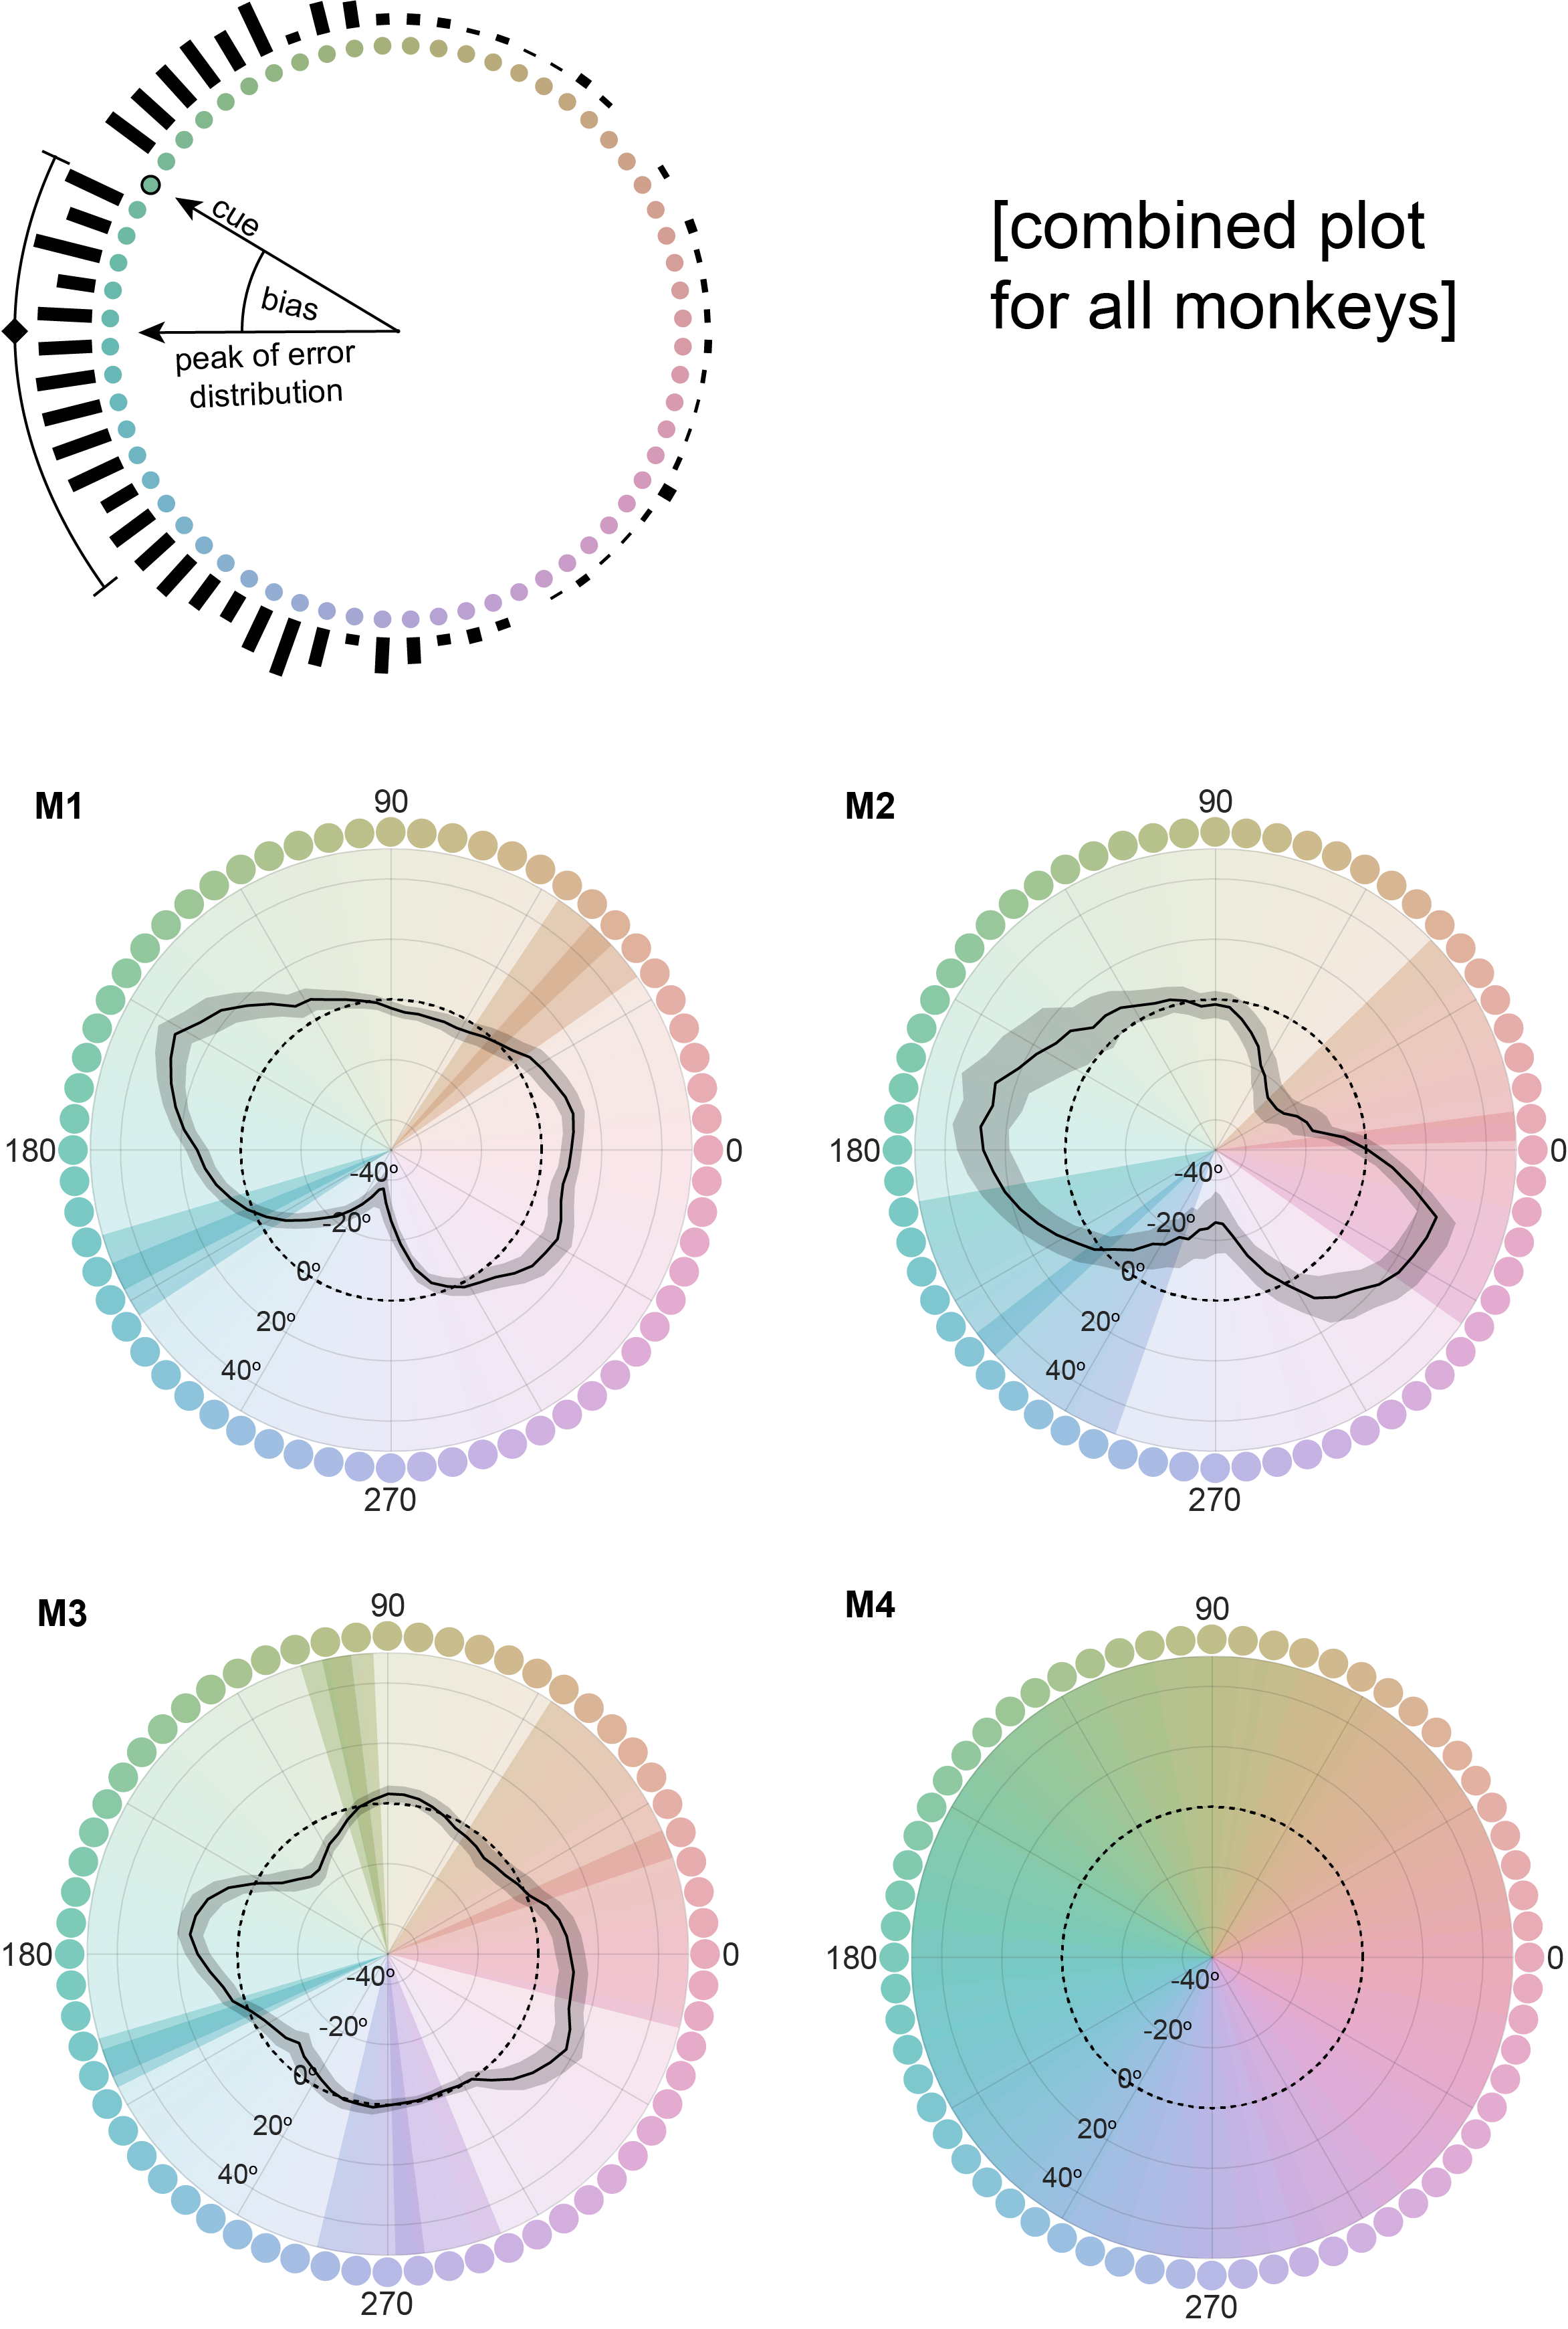
\includegraphics[height=\textwidth]{../../Figures/F3_BiasCurves_v2.png}
\end{center}
\caption{\textbf{Bias as a function of hue.} 
\emph{A.} The distribution of incorrect choices for cue \#28 for M1, with an arrow indicating the peak of a Gaussian fitted to these values which is taken as the bias for this cue. Confidence interval refers to the 95\% confidence interval on the peak of the Gaussian from the fitting procedure.
\emph{C-F.} Individual bias curves for the 4 tested animals.
\emph{Black dotted line:} The zero lines where responses would fall if there were no biases.
\emph{Black line:} Bias as a function of hue for monkeys M1, M2, M3 and M4, smoothed with a moving average filter of 5 cues. 
\emph{Gray filled:} confidence intervals for the line, computed through bootstrapping . 
\emph{Colored radiating line:} Median attractor point from bootstrap procedure.
\emph{Colored wedge:} Confidence intervals for the 2.5\% and 97.5\% percentiles for the bootstrapped attractor points.
See Methods for further details.} % CIELUV. Hues approximate.
\label{fig:BiasCurves}
\end{figure}


\paragraph{Shared color categories across monkeys.}

We see that all tested monkeys share two common attractor points, which we interpret as evidence of two shared color categories: a warm/orange-ish category (between 0$^\circ$ and 45$^\circ$), and a cool/blue-ish category (between 180$^\circ$ and 225$^\circ$).

\paragraph{Individual differences between monkeys.}

In one animal we see evidence of additional categories: strong evidence for a greenish category and weak evidence for a purple category (the ``strength" of a category can be gleaned from looking at the local gradient at the zero-crossing point)

% Results table?


\paragraph{Learning rates/DKL.}

\paragraph{Independent verification of found categories.}

\paragraph{Longitudinal analysis - power analysis and progression over time.}

Segmenting our data into subgroups of 5000 datapoints allowed us to both look at whether the determined categories varied over time, and also allowed us to perform a rough power analysis. From the monkeys studied it was clear that during our data collection period the categories remained static (within our measurement uncertainty), and also that the categories we saw are reliable enough to be seen with substantially less data. See Figures XXX % \autoref{}


%\begin{figure}
%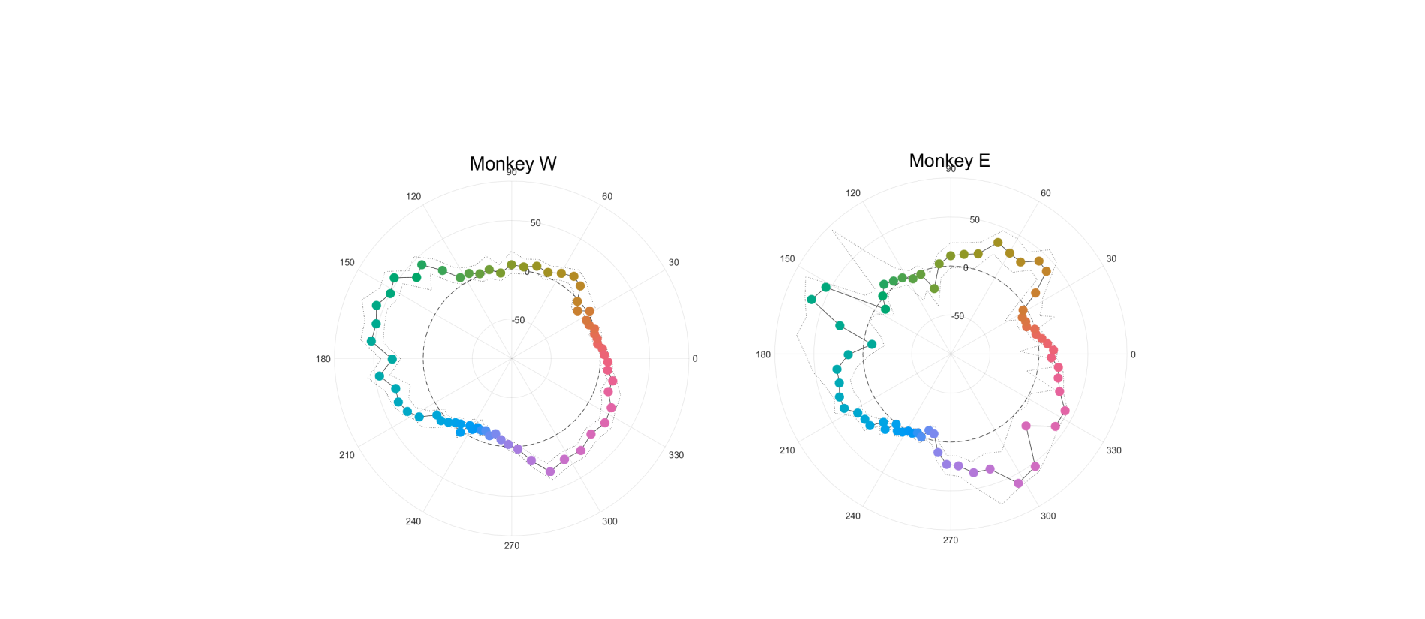
\includegraphics[width=\textwidth]{../../Figures/Old/panichellobias.pdf}
%\caption{Bias as a function of hue, for Panichello monkeys} 
%\end{figure}


